% Appendix A

\chapter{Manuel - Commission INFO} % Main appendix title

\label{AppendixA} % For referencing this appendix elsewhere, use \ref{AppendixA}


\section{Introduction}
Le but de présenter un scénario typique d'utilisation pour la \textbf{commission INFO}. L'application au moment où ce scénario a été conçu n'est pas encore finie. Il risque d'y avoir des changements au niveau de son design et l'ajout de certaines \textit{features} non encore implémentées (comme la gestion des utilisateurs, ou certaines contraintes spécifiques). Cependant, la base de l'application est suffisamment présente que pour permettre à ce test d’être pertinent.

Le scénario est le suivant. Tout d'abord, le lecteur va être amené à créer un graph avec l'outil yEd. Ensuite, il va l'importer dans l'implication. Après, il va rajouter des données au catalogue de cours précédemment créé. Il sera ensuite expliquer comment accéder aux différents vues montrant les données qui ont été importée (comme les cours, les modules, ...). Enfin, il sera présenter comment créer des programmes de cours à partir des données importées.



Bon amusement :-)

P.S. Le lien vers l'application : \url{http://curriculum-mgmt.herokuapp.com/}
\subsection{Feedback recherché}
\begin{itemize}
\item Des bugs s'il y en a
\item Critiques au niveau de l'interface, des étapes qui ne sont pas claires, etc
\item Features manquantes dans l'application
\item Attributs identifiants certains modèles qui ne sont pas adéquats. (Pour les catalogue par exemple, je ne suis pas sûr que la faculté et le département soit pertinents
\item ...
\end{itemize}
\section{Gestion des catalogues de cours}
\subsection{Page d'accueil}

\begin{figure}[H]
\centering

\includegraphics[width=\textwidth]{landing_page_access_to_catalog}
\caption{Accès de gestion des catalogues}
\label{fig:landing_page_catalog}
\end{figure}

Sur l'image ~\ref{fig:landing_page_catalog} apparaît la page d'accueil Le menu pour accéder aux différents catalogues de cours est entouré d'un cadre rouge sur la capture d'écran.

\subsection{Accéder aux catalogues}
Après avoir cliquer sur le menu catalogue, nous arrivons sur la page montrant les différents cours présents dans l'application. Comme vous pouvez le voir sur la capture d'écran ~\ref{fig:catalog_index}, il n'y a qu'un seul catalogue pour le moment dans l'application. Vous pouvez cliquer sur le bouton \textit{Plus d'informations} pour accéder au catalogue en question, ou encore sur \textit{supprimer} pour le supprimer de l'application. Cependant, nous allons commencer par créer un graphe pour pouvoir créer un catalogue en l'important\\

\begin{figure}[H]
\centering
\caption{Liste des catalogues}
\label{fig:catalog_index}
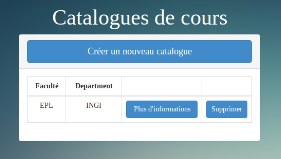
\includegraphics[scale= 1]{catalog_index}
\end{figure}

\subsection{Création d'un graphe de cours avec yEd}
\subsubsection{Le menu de yed}
Dans cette section nous allons pas à pas construire un graph de cours avec yed (L'outil utilisé pour générer des graphes).

Yed est disponnible ici \url{http://www.yworks.com/en/downloads.html\#yEd}

Nous allons créer un petit catalogue de cours, composé d'un programme, un module quelques cours et quelques dépendances. Tout d'abord, ouvrez le programme yEd et créer un nouveau document. Une fois le yEd ouvert et le nouveau graph créer, vous verrez à votre droite le menu suivant ~\ref{fig:yed_menu}.

\begin{figure}[H]
\centering
\caption{Menu de yEd}
\label{fig:yed_menu}
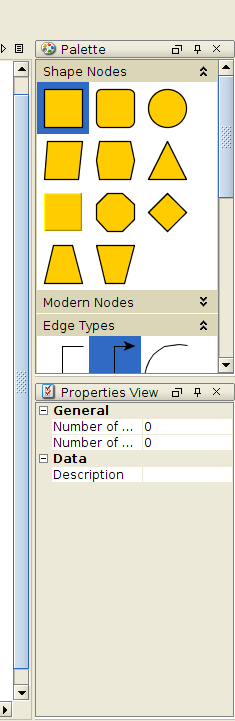
\includegraphics[scale=0.5]{yed_menu}
\end{figure}


\subsubsection{Créer des cours}
Pour créer les objets représentant les cours, il faut utiliser ce menu ~\ref{fig:yed_node_menu} et sélectionner le carré (en \textcolor{blue}{bleu sur la capture d'écran}) puis cliquer sur le document pour l'ajouter au graphe.

\begin{figure}[H]
\centering
\caption{Menu de création des noeuds}
\label{fig:yed_node_menu}
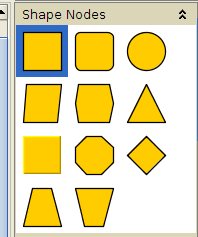
\includegraphics[scale=0.6]{yed_node_menu}
\end{figure}

Pour nommer le nœud:
\begin{enumerate}
\item Clique droit sur le nœud
\item Cliquez sur \textit{properties}
\end{enumerate}

Le menu suivant apparaîtra ~\ref{fig:properties_menu}. Il suffit de remplir le champ \textit{Texte} avec le nom désiré.

\begin{figure}[H]
\centering
\caption{Ajouter un nom à un noeud}
\label{fig:properties_menu}
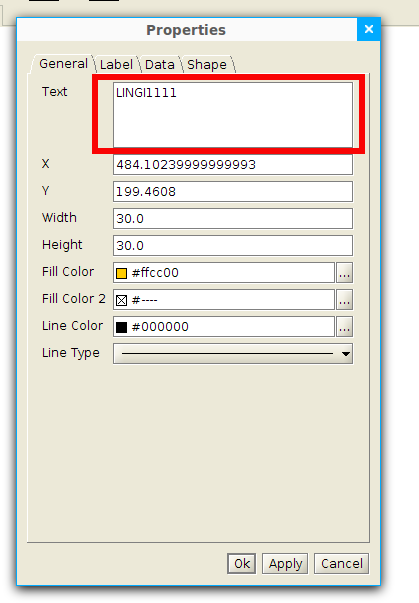
\includegraphics[scale=0.6]{properties_menu}
\end{figure}


\subsubsection{Ajouter des dépendances}

Pour représenter les dépendances entre les cours, il faut utiliser le menu présent sur l'image  ~\ref{fig:yed_edge_menu} qui permet de dessiner des arrêtes entre les nœuds.

\begin{figure}[H]
\centering
\caption{Menu de création d'arrêtes}
\label{fig:yed_edge_menu}
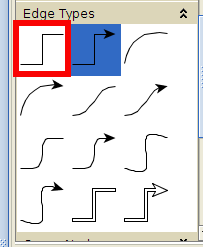
\includegraphics[scale=0.6]{yed_edge_menu}
\end{figure}

Nous utilisons deux type d'arrêtes;

\begin{itemize}
\item en \textcolor{blue}{bleu} sur l'image ~\ref{fig:yed_edge_menu}, les arrêtes pour représenter les prérequis
\item en \textcolor{red}{rouge} sur l'image ~\ref{fig:yed_edge_menu}, les arrêtes pour représenter les corequis
\end{itemize}

En créant un catalogue de deux cours, avec l'un étant le prérequis de l'autre, nous obtenons le graph présent sur l'image suivante ~\ref{fig:dependancies_example}.

\begin{figure}[H]

\label{fig:dependancies_example}
\centering
\caption{Deux cours avec une dépendance}
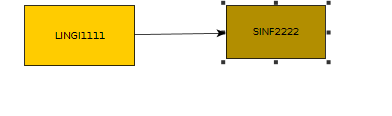
\includegraphics[scale=0.5]{dependancies_example}

\end{figure}

\subsubsection{Insérer des cours dans des modules}
Après avoir créer plusieurs cours, il est possible de regrouper ces nœuds dans une boite.
\begin{enumerate}
\item Sélectionner les noeuds à regrouper
\item Clique droit
\item Cliquer sur \textit{grouping}
\end{enumerate}

Vous obtiendrez une boite comme sur la capture ~\ref{fig:node_grouping}

\begin{figure}[H]
\centering
\caption{Mettre des nœuds dans une boite}
\label{fig:node_grouping}
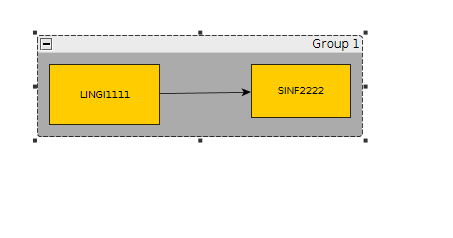
\includegraphics[scale=0.5]{node_grouping}
\end{figure}

La démarche à suivre pour nommer les boites est la même que celle pour nommer les nœuds.

Avant de poursuivre, il est nécessaire de préciser la structure de graph reconnue par l'application. 

\begin{itemize}
\item Un \textbf{catalogue} est représenté par un \textbf{graphe} et est composé exclusivement de \textbf{programmes}
\item Un \textbf{programme} est représenté par une \textbf{boite} et est composé de \textbf{modules} et de \textbf{cours}
\item Un \textbf{module} est représenté par une \textbf{boite} et est composé de plusieurs \textbf{sous-modules} et \textbf{cours}
\item Un \textbf{sous-module} marquera dans l'application tout les \textbf{cours} qu'il contient comme obligatoire pour le \textbf{module} parent.
\item Un \textbf{cours} est représenté par un \textbf{nœud} et peut avoir plusieurs dépendances. 
\item Une \textbf{dépendance} est représenté par une \textbf{arrête} entre deux \textbf{nœuds}.(Elle peut avoir deux type comme expliqué plus tôt
\end{itemize}

Sur l'image \ref{fig:small_catalog_example}, vous pouvez voir un exemple de catalogue valide.

\begin{figure}[H]
\centering
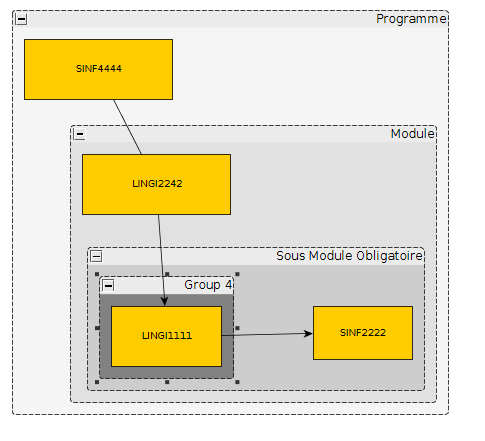
\includegraphics[scale=0.6]{small_catalog_example}
\label{fig:small_catalog_example}
\caption{Un (petit) catalogue de cours valide}

\end{figure}

\subsection{Import du graph dans l'application}
Pour poursuivre, vous pouvez soit utiliser le graphe que vous venez de créer avec yEd, soit télécharger un graph complet à l'adresse suivante : \url{http://xavier.ethylix.be/graph.graphml}

Vous êtes donc sur la page comme illustré sur l'image \ref{fig:catalog_new}.

\begin{figure}[H]
\centering
\caption{Création d'un catalogue de cours}
\label{fig:catalog_new}
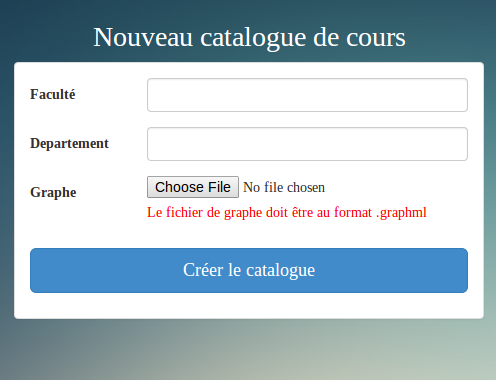
\includegraphics[scale=0.6]{catalog_new}
\end{figure}

Remplissez, les champs, sélectionner le fichier de graph désiré et cliquez sur \textit{Créer le catalogue}

Vous arrivez sur la page présentée sur l'image suivante \ref{fig:catalog_show}

\begin{figure}[H]
\centering

\caption{Le catalogue une fois créé}
\label{fig:catalog_show}
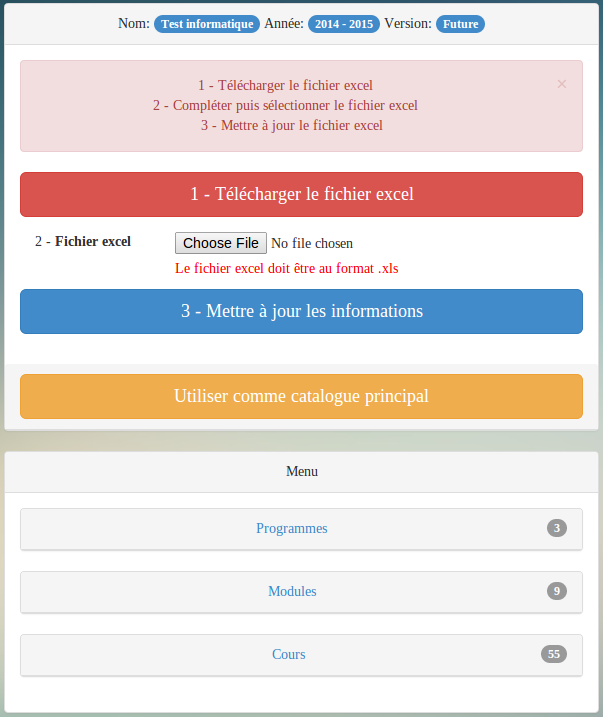
\includegraphics[width = \textwidth]{catalog_show}
\end{figure}

\subsubsection{Mise à jour des informations contenues dans le catalogue}
Les informations contenues dans le graphe ne sont pas complète. C'est pourquoi il est possible (et même fortement conseillé d'en ajouter via un formulaire excel

Pour ce faire il est conseillé  de commencer par télécharger le formulaire excel (en cliquant sur le bouton en \textcolor{red}{rouge} sur l'image \ref{fig:catalog_show}) contenant les informations du catalogue ainsi que certaines proposition d'attributs à ajouter au catalogue. Il est préférable de ne pas passer cette étape. Dans le cas contraire, vous serez obligé d'écrire les identifiants de tout les différents programmes, modules et cours un à un dans le formulaire. Pour un catalogue de 55 cours, cela peut être long. 

Une fois le \textit{template} de formulaire téléchargé et complété , sélectionnez le et cliquez sur le bouton \textit{Mettre à jour les informations} (en \textcolor{blue}{bleu} sur l'image \ref{fig:catalog_show}).

\subsection{Création de programme de cours}

Il est possible de créer des programmes \textit{à la carte} avec les modules et différents cours importés dans l'application lors de l'import de graphe. Pour ce faire, cliquer, dans le menu à droite sur le lien intitulé \textit{Programme} (Image \ref{fig:catalog_show}).

Vous arriverez sur une page comme présentée sur l'image \ref{fig:program_index} qui liste tout les programmes présent dans le catalogue. Vous pouvez inspecter les modules et les cours dont il est composé en cliquant sur le bouton \textit{Plus d'informations}, ou même le supprimer.

\begin{figure}[H]
\centering
\caption{Programmes créés par défaut}
\label{fig:program_index}
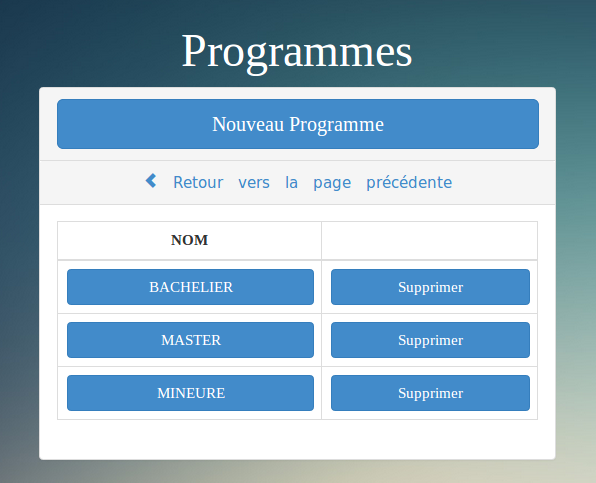
\includegraphics[width = \textwidth]{program_index}

\end{figure}

Pour créer un programme, il suffit de cliquer sur le  bouton \textit{Créer un programme}. Vous arriverez sur la page illustré sur l'image \ref{fig:catalog_new}

\begin{figure}[H]
\centering
\caption{Création programme "à la carte"}
\label{fig:program_new}
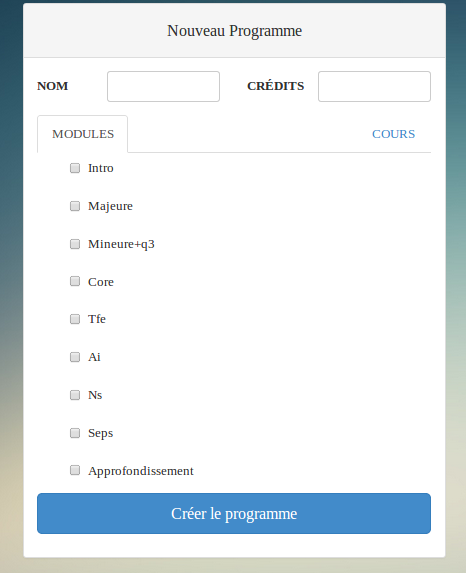
\includegraphics[width = \textwidth]{program_new}
\end{figure}

Remplissez les différents champs et naviguez entre les onglets \textbf{MODULES} et \textbf{COURS} pour choisir les modules et cours dont le nouveau programme sera composé. Cliquez ensuite sur \textit{Créer le programme}. Vous arriverez à la page illustrée sur l'image~\ref{fig:program_show}. En cliquant sur le menu déroulant intitulé \textit{Menu}, vous pouvez accéder aux différents modules et sous-modules qui le compose. 

\begin{figure}[H]
\centering
\caption{Le programme une fois créé}
\label{fig:program_show}
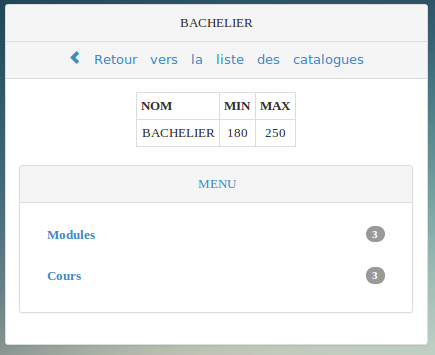
\includegraphics[width = \textwidth]{program_show}
\end{figure}

\section{Gestion des requêtes de validations}
Lorsqu'un étudiant désire envoyer le programme qu'il s'est créé à la validation, une demande de validation est envoyé à la \textbf{commission INFO}. Pour accéder à ces demandes de validations, 
il suffit de cliquer sur le menu intitulé \textit{Validations} entouré en rouge sur l'image \ref{fig:landing_page_access_to_validations}.

\begin{figure}[H]
\centering
\caption{Accéder aux demandes validations}
\label{fig:landing_page_access_to_validations}
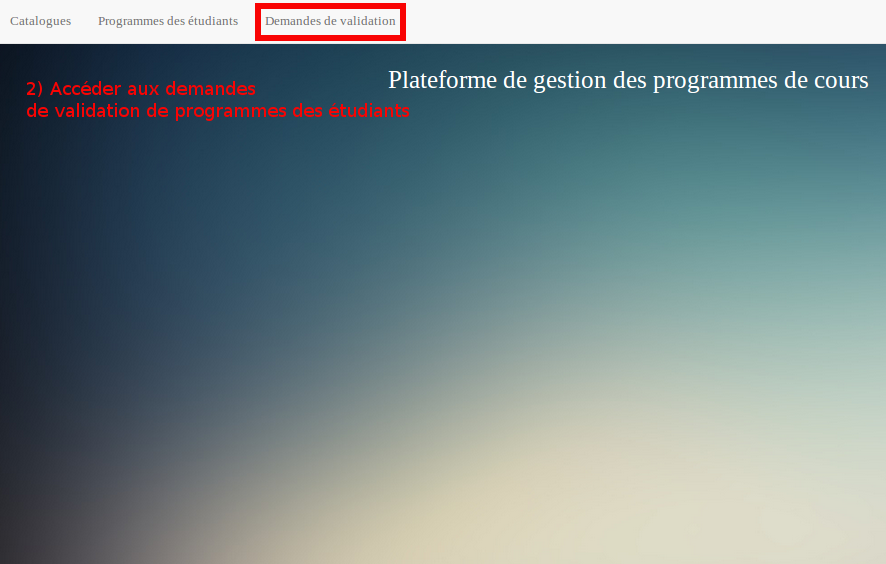
\includegraphics[width=\textwidth]{landing_page_access_to_validations}
\end{figure}

Sur la page des validations (Image~\ref{fig:validations}) vous pouvez
\begin{itemize}
\item inspecter le programme que l'étudiant demande de valider en cliquant sur \textit{Programme} (en \textcolor{blue}{bleu} sur l'image \ref{fig:validations})
\item valider la requête en cliquand sur \textit{Valider} (en \textcolor{green}{vert} sur l'image \ref{fig:validations})
\item refuser la requête en cliquant sur \textit{Refuser} (en \textcolor{red}{rouge} sur l'image \ref{fig:validations})
\end{itemize}

\begin{figure}[H]
\centering
\caption{Quelques demandes de validations}
\label{fig:validations}
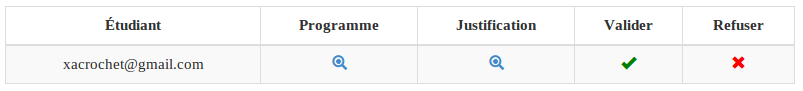
\includegraphics[scale=0.6]{validations}

\end{figure}